\documentclass{umm-senior-sem}
\usepackage{cite}
\usepackage{url}

%\usepackage{setspace}
%\setstretch{2} 
\begin{document}
\title{Summary of Using Ant Colony Optimizations to Learn Fuzzy Cognitive Maps}
\author{
\alignauthor
Chris Aga \\
\affaddr{ 
University of Minnesota, Morris \\
600 East 4th St. \\	
Morris, Minnesota 56267} \\
\email{agaxx010@morris.umn.edu}
}

\maketitle

\begin{abstract}
This paper summarizes the application of Ant Colony Optimizations (ACO) to model accurate relationships between multiple concepts in a system when expert knowledge is lacking. The model used in~\cite{main:2012} by Ye Chen is termed Fuzzy Cognitive Map. It consitsts of nodes (concepts) with weighted edges which represent the magnitude of exhibition or inhibition of all concepts towards each other. Chen gives a brief summary on FCMs, approaches to learning of FCMs in particular ACO and compares their efficiencies to one another. This paper attempts to explain in more accurate detail each of the concepts covered in Chen's paper.
\end{abstract}

\keywords{Fuzzy Cognitive Maps, Ant Colony Optimization, numerical optimization, data-driven learning algorithm}

\section{Introduction}
\label{sec:intro}
Accurate models of relationships and interactions between genes in a cell can be hard to generate due to lack of expert knowledge. Typically, a passable amount of knowledge is available on determining relationships between concepts such as genes in a cell, Fuzzy Cognitive Maps (FCM) are a common model used to represent these relationships because of their readability and ability to handle logic in a approximated form. Typically, enough expert knowledge is known to generate a tolerable FCM, and from there, a learning technique is used to improve the accuracy of an FCM. Even though a large abundance of data on the particular state of genes at many moments are available, still, without proper knowledge, developing accurate causal relationships between each concept is nontrivial. This is where the learning of FCMs with randomly generated relationships between elements or concepts is important. Ye Chen in~\cite{main:2012} investigates the use of Ant Colony Optimizations (ACO) as a solution to this problem. 

The following section will give a brief overview of what a Fuzzy Cognitive Map is, describe the purpose of "learning" a Fuzzy Cognitive Map and comment on current learning approaches. The overall model of Ant Colony Optimizations and its application to the learning of Fuzzy Cognitive Maps will be explained in depth in Section~\ref{sec:aco}. Finally, Section~\ref{sec:comparison} will compare the previously discussed learning approaches to Ant Colony Optimization as a learning approach.

\section{Learning of Fuzzy Cognitive Maps}
\label{fcm}
\subsection{Fuzzy Cognitive Maps Background}
A Fuzzy Cognitive Map (FCM) is an object which represents real valued causal relationships (represented by a weighted edge) between concepts (nodes) in a system. An example is depicted in~\ref{fig:fcm} and describes the relationships that: life-span, average body weight, amount of food present among a population, and population-size have with each other. 
\begin{figure}
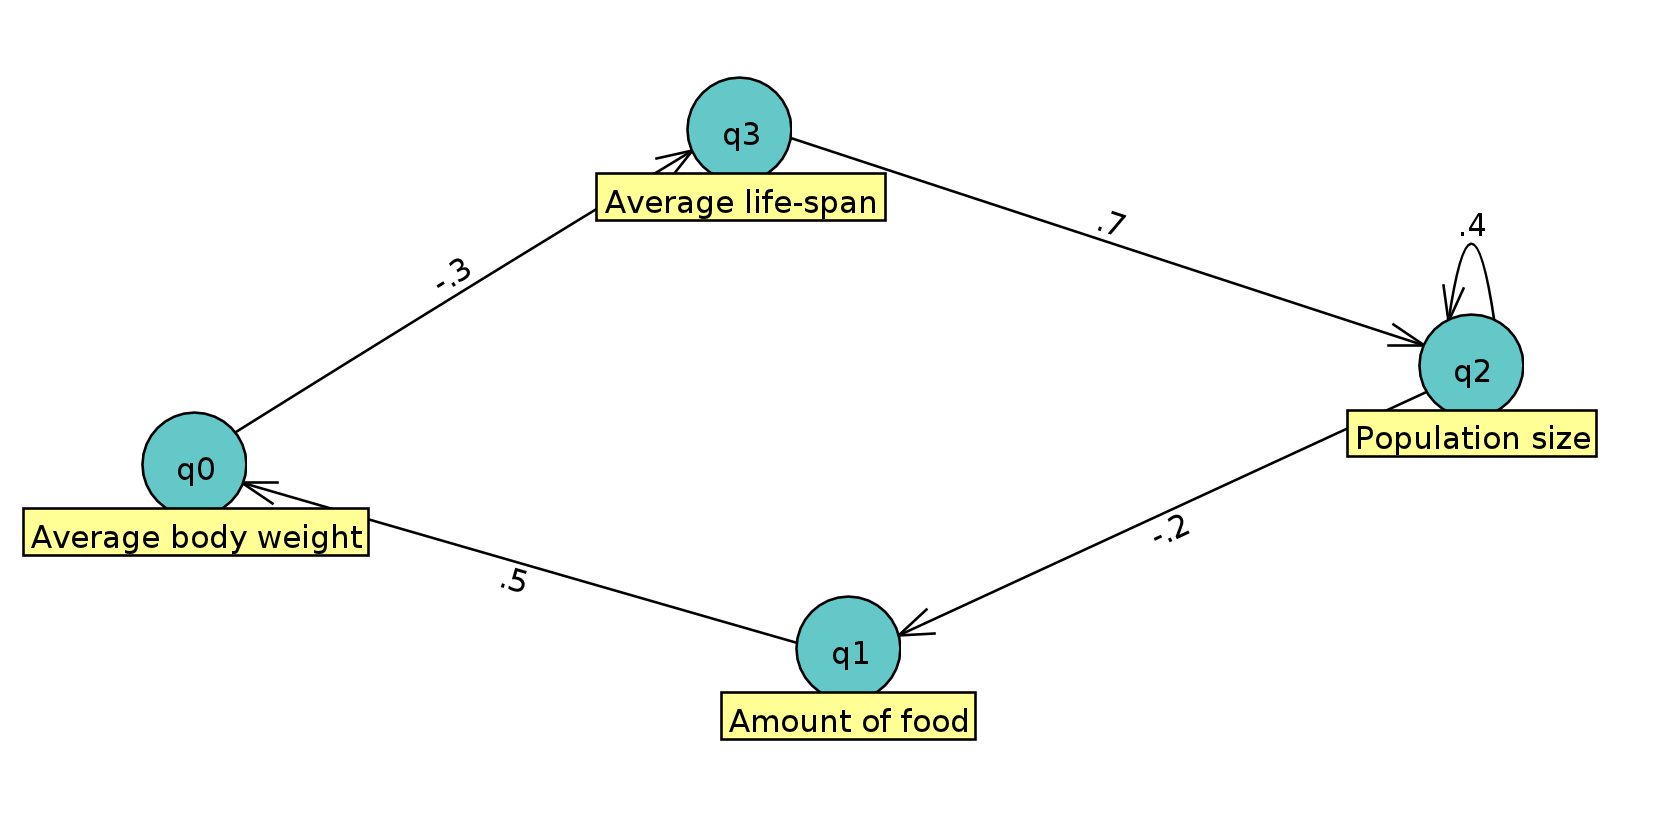
\includegraphics[scale=0.15]{images/population.png}
\label{fig:fcm}
\caption{Example of a Fuzzy Cognitive Map representing concepts that affect each other among a population of people}
\end{figure}
FCMs in a very general sense attempt to discover the "what if" value of each concept when concepts are affected from input data~\cite{FCMbg:1999}. This is described by the activation degree of a concept which is calculated by taking the sum of each concepts' current value, multiplied by its weight edge pointing towards the concept we're attempting to find the activation degree of. The activation degree is finally calculated by applying a sigmoid function (where $\lambda$ represents a user-defined parameter to "characterize the steeepness of the function around zero~\cite{main:2012}), Equation~\ref{eq:sig} to the summation. This value is then saved to the node, this occurs for each node simultaneously.
\begin{equation}
\label{eq:sig}
 f \big(x\big) = \frac{1}{1+ e^{-\lambda x} } 
\end{equation}

\subsection{Concept of learning and its Importance}
The idea of "learning" in an FCM attempts to improving either an FCM generated with some expert knowledge backing or a randomly generated FCM. By the end of the learning process, at each interval, the FCM should be able to output very similar outputs to the data it was learned with. This paper summarizes 2 techniques used for learning, and gives an in depth explination of a fourth approach termed Ant Colony Optimization (ACO). 

\subsection{Current techniques used for FCM learning}
A major approach used for learning of Fuzzy Cognitive Maps is termed nonlinear Hebbian learning. This model approaches learning in a similar way to how neurons interact and activate during learning in the brain~\cite{response:2003}. Hebbian learning is based on synchronous firing of neurons, neurons (represented as concepts in this system) next to each other directly affect one another. If two concepts are activated simultaneously, this represents the strengthening relationship between two concepts, which is analagous to neuron plasticity in the brain. Stach explains in~\cite{nhl:2008} that updating change in weights of one concept to another when a "neuron" fires is best approached by applying the product of the adjacent concepts' weights to one another. A pitfall in this approach is the possibility of reaching infinite growth, but a forgetting term is used to keep the weights in the predefined bounds. 

Another common approach, termed Real Coded Genetic Algorithm (RCGA) is a Genetic Algorithm approach using real numbers to minimize the error of an FCM's output compared to the actual output data used to learn the FCM.

\section{Ant Colony Optimizations}
\label{sec:aco}
Ant Colony Optimization (ACO) is a technique based off of the behaviour of ants attempting to gather food to bring back to their anthill~\cite{main:2012}. When ants look for food, they leave pheromone trails behind and the more a path is traveled, the greater amount of pheromone will be left behind. Shorter paths will be traveled more by a single ant, thus it will have more opportunities to leave behind pheromones, so over time, ants will discover various shortest paths between food sources and their home. This concept is applied to the learning of Fuzzy Concept Maps (FCM) by atttempting to minimize the error between the generated output of an FCM and the actual output data that was used to initially enhance the FCM. 

Each ant in the population takes what is called a "tour", this involves travelling from each node, to every other node (self inclusive) in the system of concepts. The entire "tour" represents an ant travelling from its home to a food source. This tour is constructed from various "checkpoints". These checkpoints are values that represent the weight of one node to the next. Again, the entire tour an ant takes is of the form: 
\begin{equation}
 \big\{w_{1,1}, w_{1,2}, w_{1,3} ... w_{n,n}\big\} 
\end{equation}
Where each $w_{i,j}$ represents the weight from $Concept_i$ to $Concept_j$.
Between each node, there are $N_d$ checkpoints, where $N_d$ is the desired precision of the weighted edged between concepts. Each checkpoint, as depicted in Figure~\ref{fig:antPath}, is a number 0-9, and between each number in a $column_i$ and every other box in the following $column_{i+1}$, a pheromone intensity is present to help guide ants along "shorter trails", or in the case of optimizing the accuracy of causality relationships between concepts in an FCM, reducing the difference between FCM concept activation values and actual values of the output data used to generated the FCM.

\section{Comparison of Fuzzy Cognitive Map Learning Approaches}
\label{sec:comparison}

\section{Conclusion}
\label{sec:Conclusion}
Conclusion.

\nocite{*}
%^this is a very important addition so that
%references will be included property

\bibliography{Bibliography}
\bibliographystyle{abbrv}
\end{document}